\subsection{Sistem Tiket}

Komponen sistem tiket dapat dibagi menjadi beberapa bagian, yaitu ticket \textit{backend}, basis data relasional, dan kluster Redis. Komponen basis data relasional dapat dibagi menjadi tiga jenis, yaitu kluster PostgreSQL dengan \textit{read replica}, kluster CitusData, dan kluster YugabyteDB. Komponen ini yang akan menjadi \textit{source of truth} dari sistem ini. Selain itu, kluster Redis digunakan untuk menyimpan data agregat ketersediaan berdasarkan area.

\begin{figure}[htbp]
    \centering
    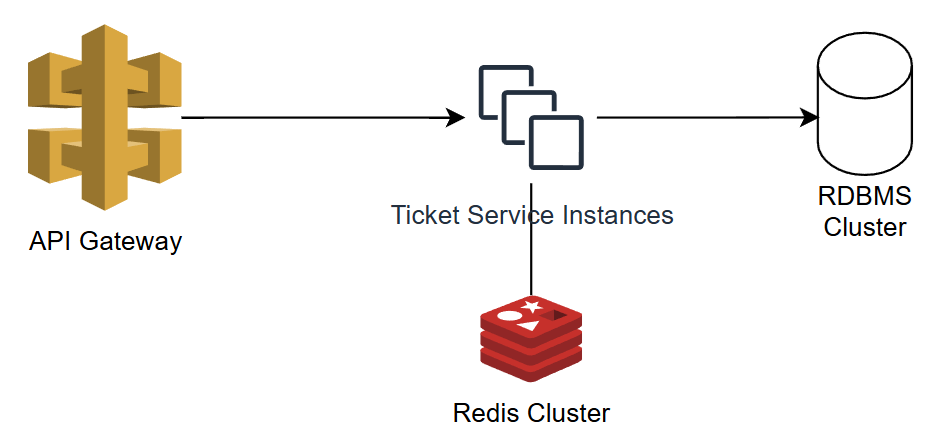
\includegraphics[width=0.8\textwidth]{resources/chapter-3/ticket-nofc.png}
    \caption{Diagram Arsitektur Sistem Tiket Tanpa \textit{Flow Control}}
    \label{fig:ticket-nofc}
\end{figure}

\pagebreak

Selain itu, berikut adalah variasi konfigurasi RDBMS yang mungkin terjadi.

\begin{figure}[htbp]
    \centering
    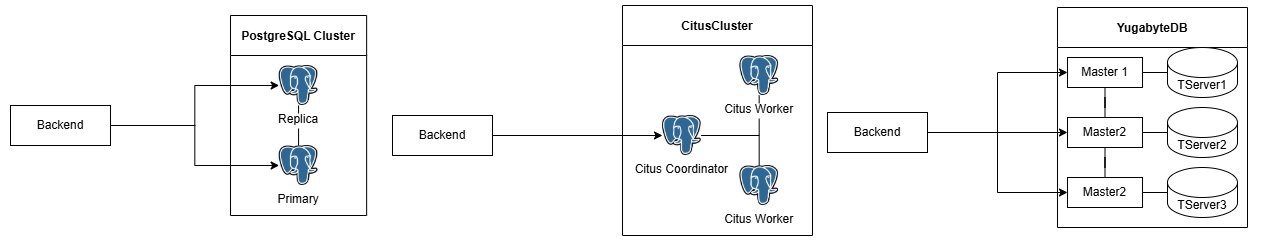
\includegraphics[width=0.5\textwidth]{resources/chapter-3/rdbms.png}
    \caption{Variasi RDBMS}
    \label{fig:rdbms-variation}
\end{figure}

Pada konfigurasi kluster PostgreSQL, klien terhubung dengan semua \textit{instance}. Pada konfigurasi CitusData, klien hanya terhubung dengan koordinator dan koordinator yang akan meneruskan permintaan kepada \textit{worker}. Pada konfigurasi YugabyteDB, klien terhubung dengan semua Master yang masing-masing terhubung dengan TServer. Klien sebenarnya dapat terhubung dengan salah satu master saja, tetapi konfigurasi seperti ini membuat koneksi klien ke YugabyteDB menjadi lebih \textit{fault tolerant} dan juga dapat mengurangi beban agar tidak terpusat pada satu \textit{instance} saja.

\begin{figure}[htbp]
    \centering
    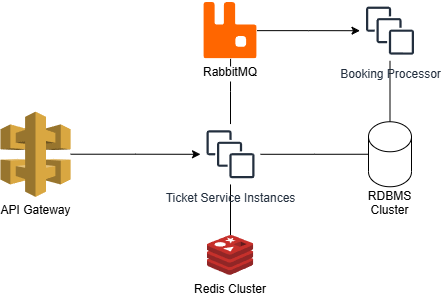
\includegraphics[width=0.8\textwidth]{resources/chapter-3/ticket-fc.png}
    \caption{Diagram Arsitektur Sistem Tiket dengan \textit{Flow Control}}
    \label{fig:ticket-fc}
\end{figure}

Pada sistem tiket dengan \textit{flow control}, terdapat dua komponen baru yaitu RabbitMQ dan \textit{booking processor}. RabbitMQ bertugas untuk menyimpan \textit{queue} permintaan pemesanan tiket dan \textit{booking processor} bertugas untuk memproses pemesanan tiket. Selain itu, kluster Redis memiliki tanggung jawab tambahan untuk menyimpan data yang digunakan untuk \textit{early dropping} permintaan pesanan yang masuk.

\pagebreak

\subsubsection{Alur Fitur \textit{Event}}

Terdapat tiga operasi pada fitur \textit{event}, yaitu membaca ketersediaan acara, membaca agregat ketersediaan area, dan membaca ketersediaan kursi. Operasi baca agregat ketersediaan area menggunakan data agregat yang dipelihara pada Redis alih-alih melakukan agregat dari basis data. Operasi baca ketersediaan kursi membaca langsung data dari basis data dengan sedikit pengoptimalan dengan menggunakan \textit{micro-caching}.

\begin{figure}[h]
    \centering
    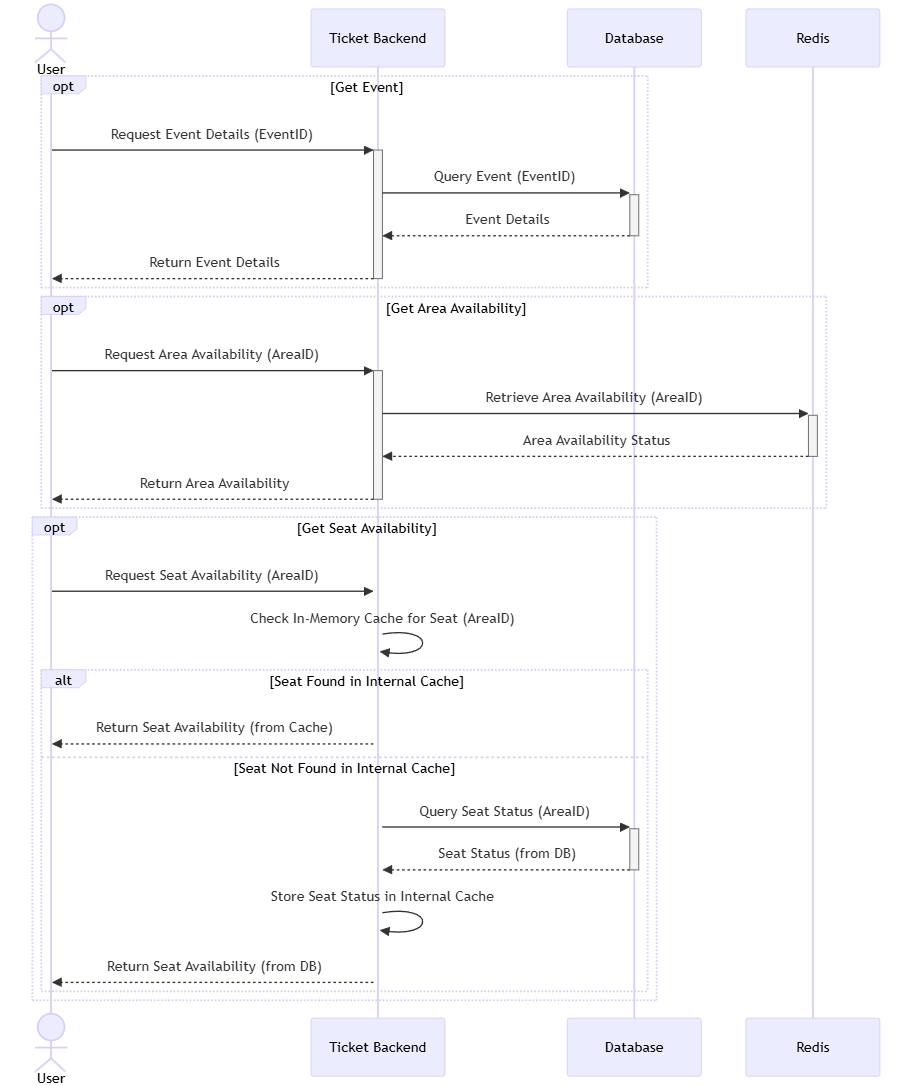
\includegraphics[width=0.9\textwidth]{resources/chapter-3/event-flow.png}
    \caption{Diagram Alur Fitur \textit{Event}}
    \label{fig:flow-event}
\end{figure}

\pagebreak

\subsubsection{Alur Fitur Pemesanan Tiket (tanpa \textit{flow control})}

Proses pemesanan tiket dimulai dengan pengguna mengirimkan permintaan pemesanan kepada sistem tiket.

\begin{figure}[h]
    \centering
    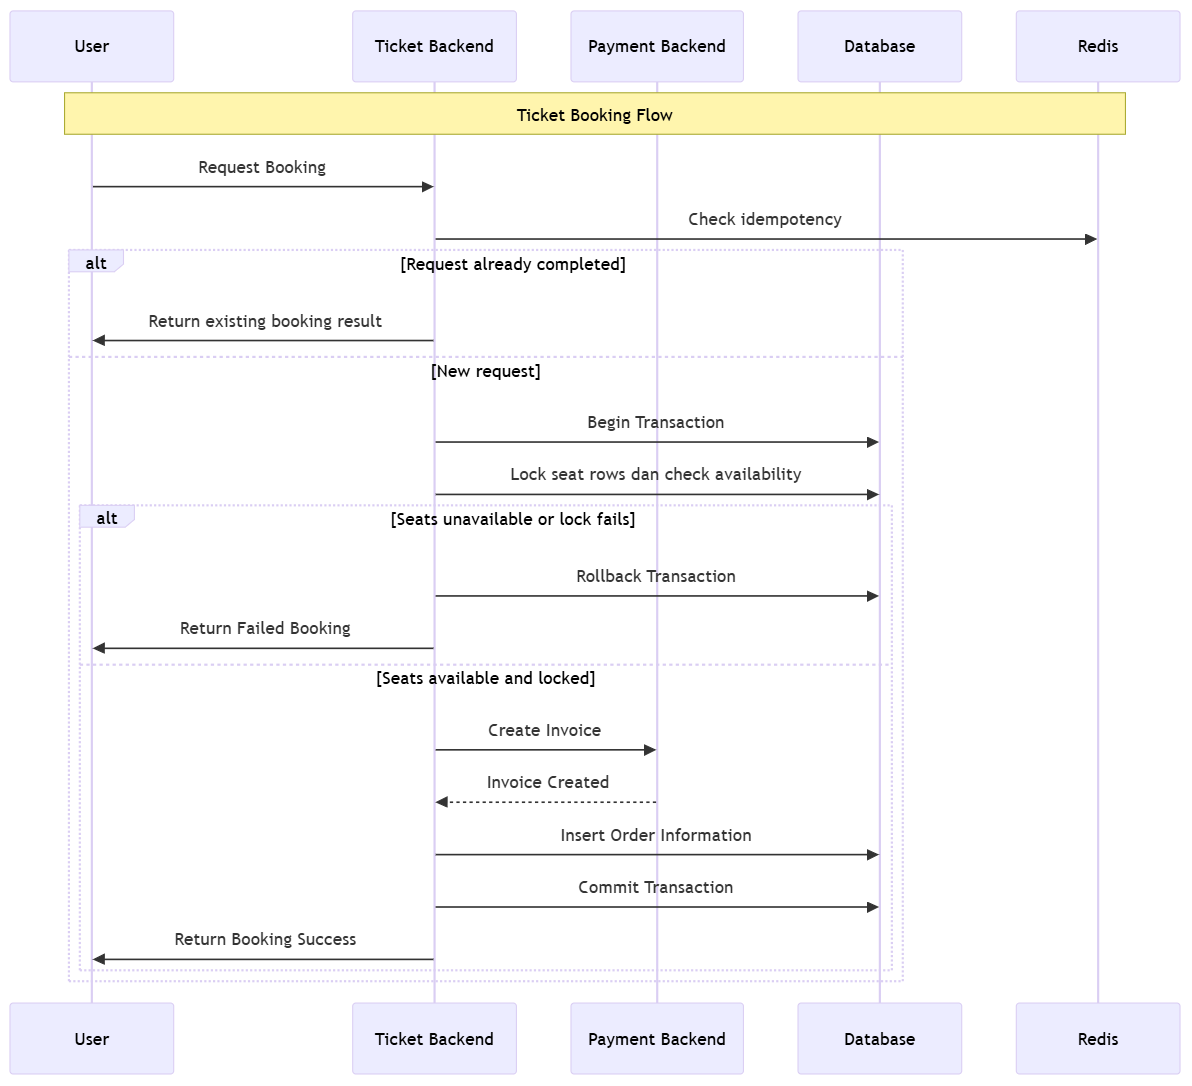
\includegraphics[width=1\textwidth]{resources/chapter-3/book-flow.png}
    \caption{Diagram Alur Fitur Pemesanan Tiket (tanpa \textit{flow control})}
    \label{fig:flow-book-flow}
\end{figure}

\pagebreak

Ketika pengguna berhasil memesan, pengguna akan melakukan pembayaran kepada \textit{payment gateway}. Setelah pembayaran selesai, pengguna memeriksa status pesanan yang telah dibuat.

\begin{figure}[h]
    \centering
    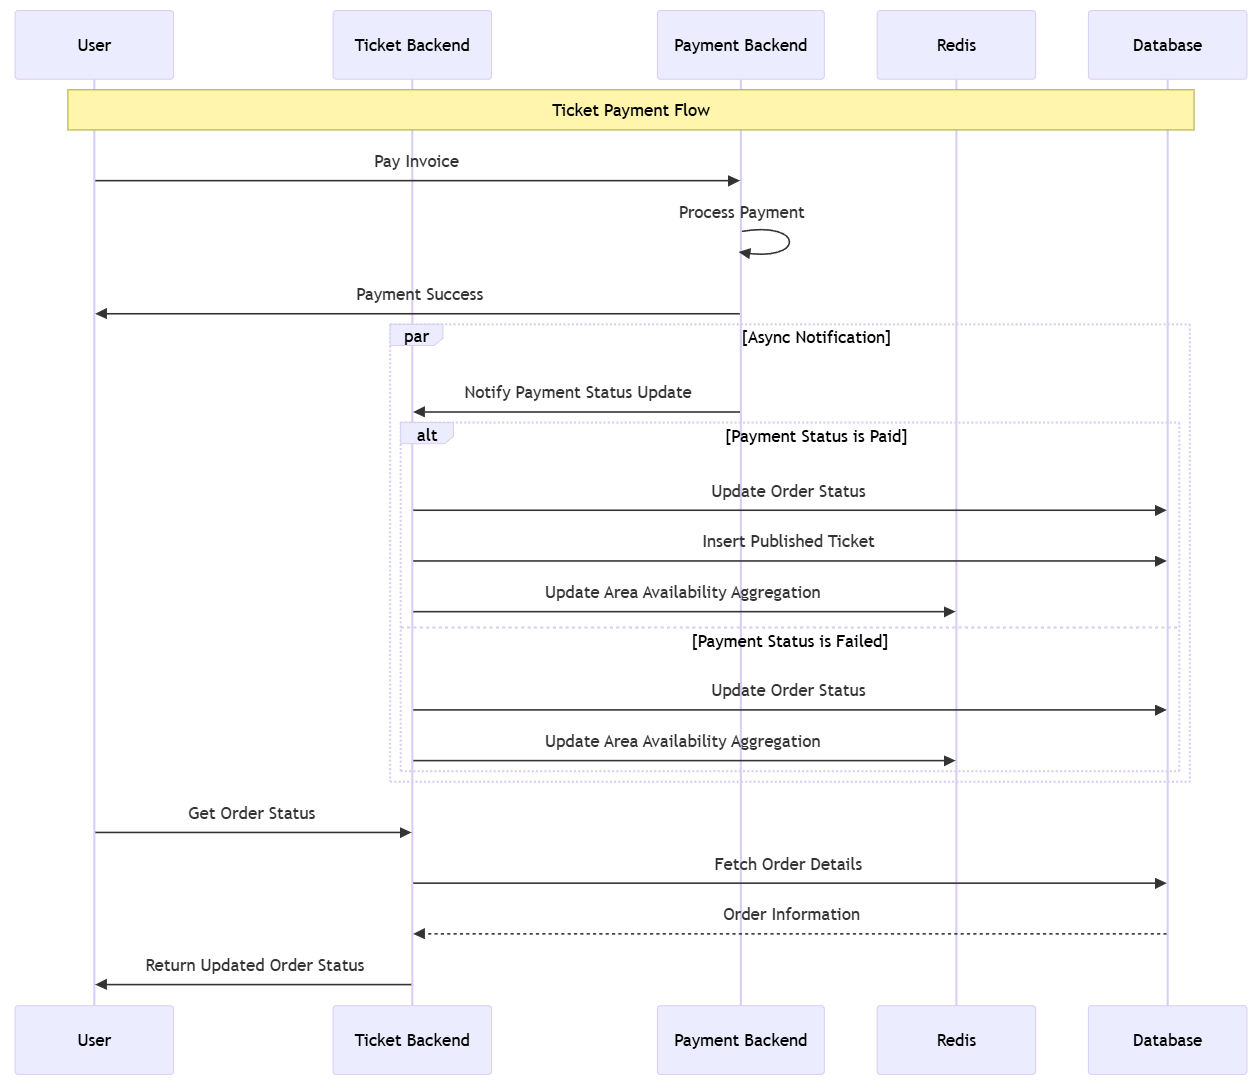
\includegraphics[width=1\textwidth]{resources/chapter-3/order-payment.png}
    \caption{Diagram Alur Fitur Pembayaran Tiket (tanpa \textit{flow control})}
    \label{fig:flow-order-payment-flow}
\end{figure}

\pagebreak

\subsubsection{Alur Fitur Pemesanan Tiket (dengan \textit{flow control})}

Proses pemesanan tiket dimulai dengan pengguna mengirimkan permintaan pemesanan kepada sistem tiket. Perbedaan dengan alur tanpa \textit{flow control} adalah penggunaan RabbitMQ dan \textit{ticket worker}. Proses pemesanan akan diproses secara \textit{partial synchrony} agar sistem dapat memproses pesanan sesuai dengan kapatiasnya. Selain itu, pendekatan ini juga memeriksa data dari \textit{early dropper} untuk menolak sebuah pesanan ketika terdapat pesanan yang sama untuk suatu kursi yang memiliki pesanan lain yang sedang diproses, tetapi belum sepenuhnya berhasil.

\begin{figure}[h]
    \centering
    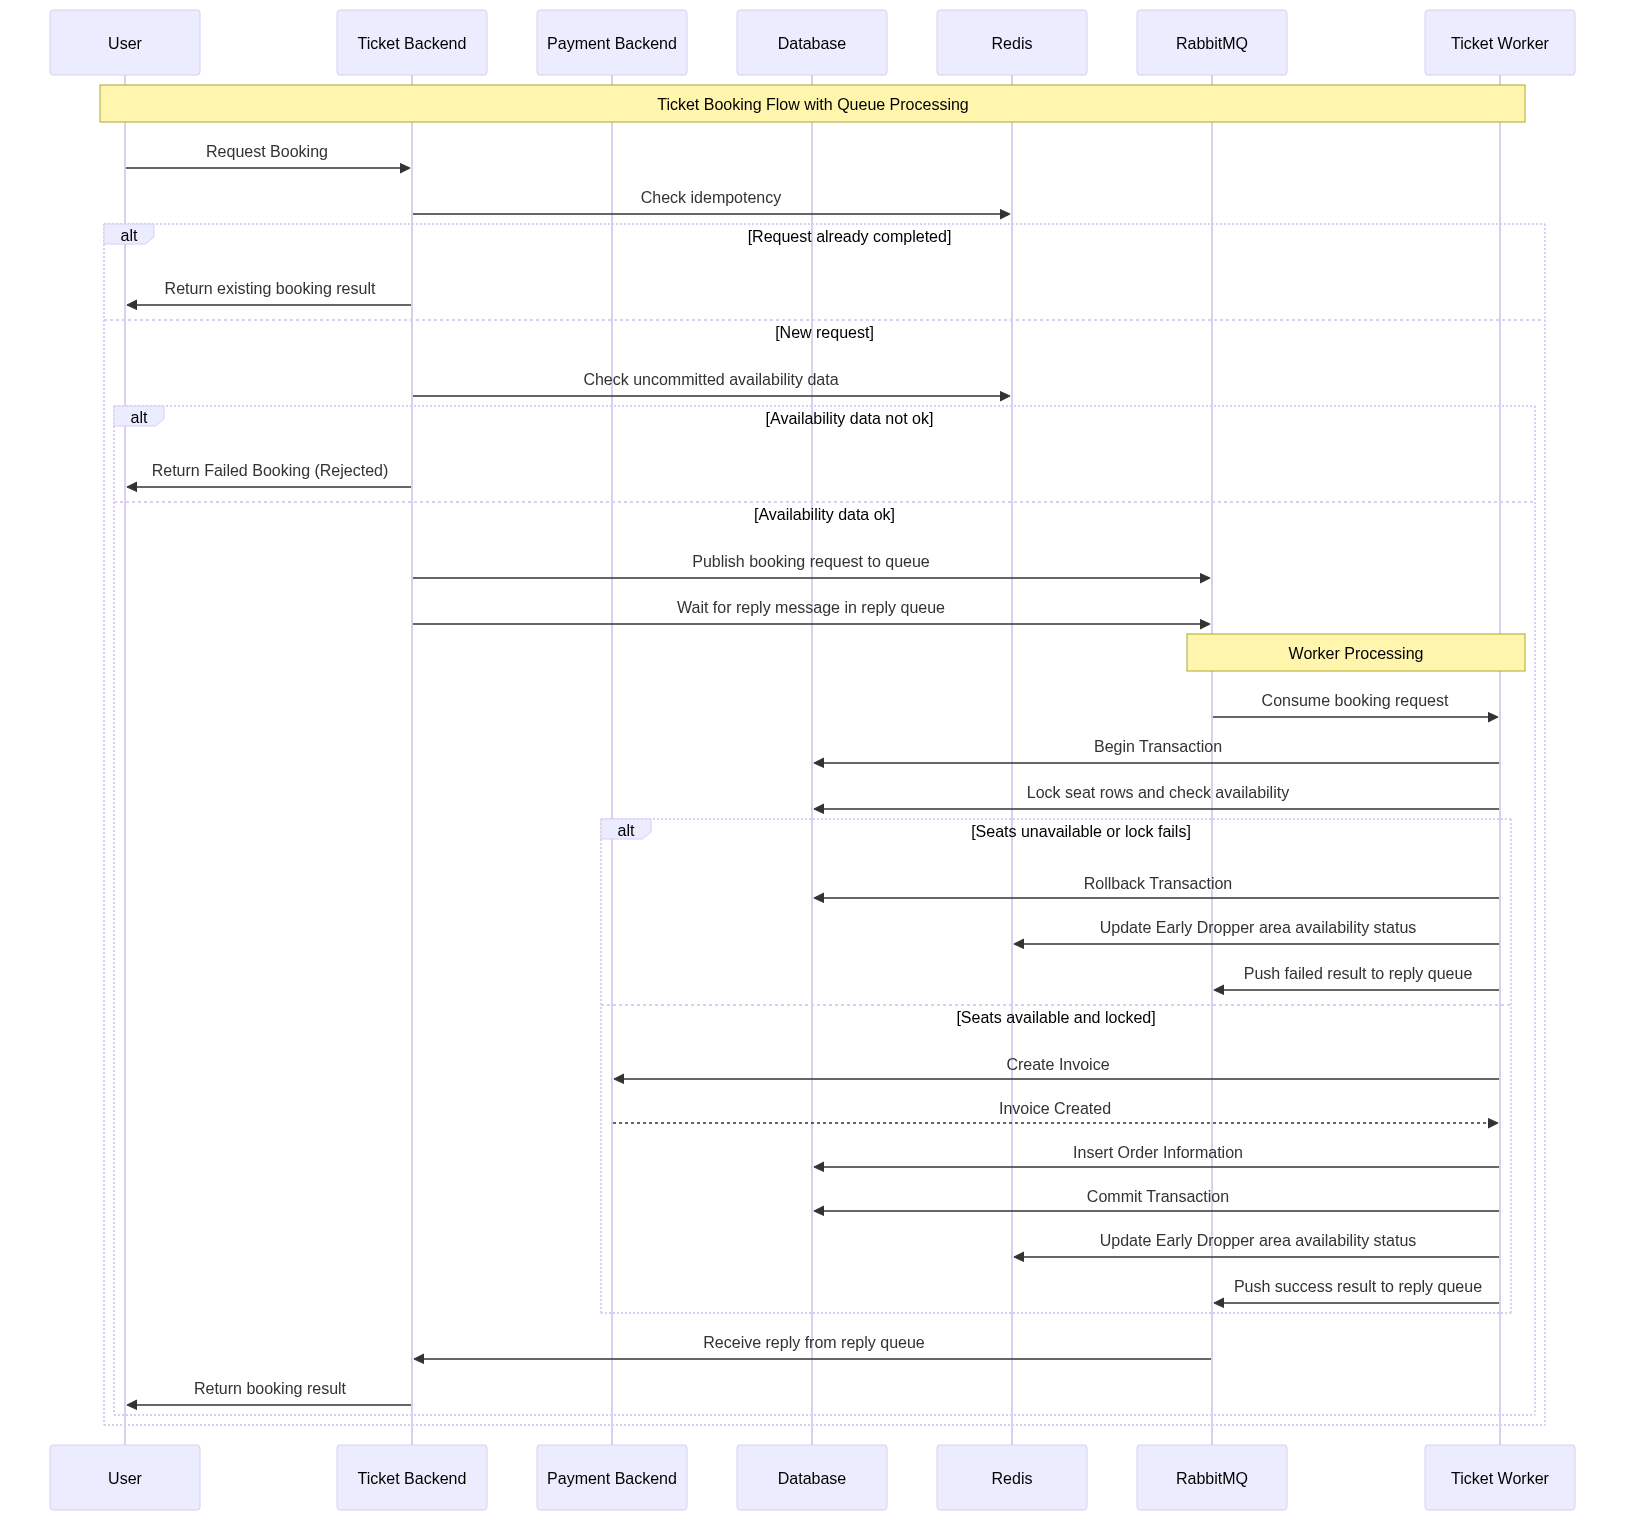
\includegraphics[width=1\textwidth]{resources/chapter-3/book-async.png}
    \caption{Diagram Alur Fitur Pemesanan Tiket (dengan \textit{flow control})}
    \label{fig:flow-book-fc}
\end{figure}

\pagebreak

Ketika pengguna berhasil memesan, pengguna akan melakukan pembayaran kepada \textit{payment gateway}. Setelah pembayaran selesai, pengguna memeriksa status pesanan yang telah dibuat. Tidak ada perbedaan signifikan selain pembaruan data pada Redis untuk sinkronisasi data pada \textit{early dropper}.

\begin{figure}[h]
    \centering
    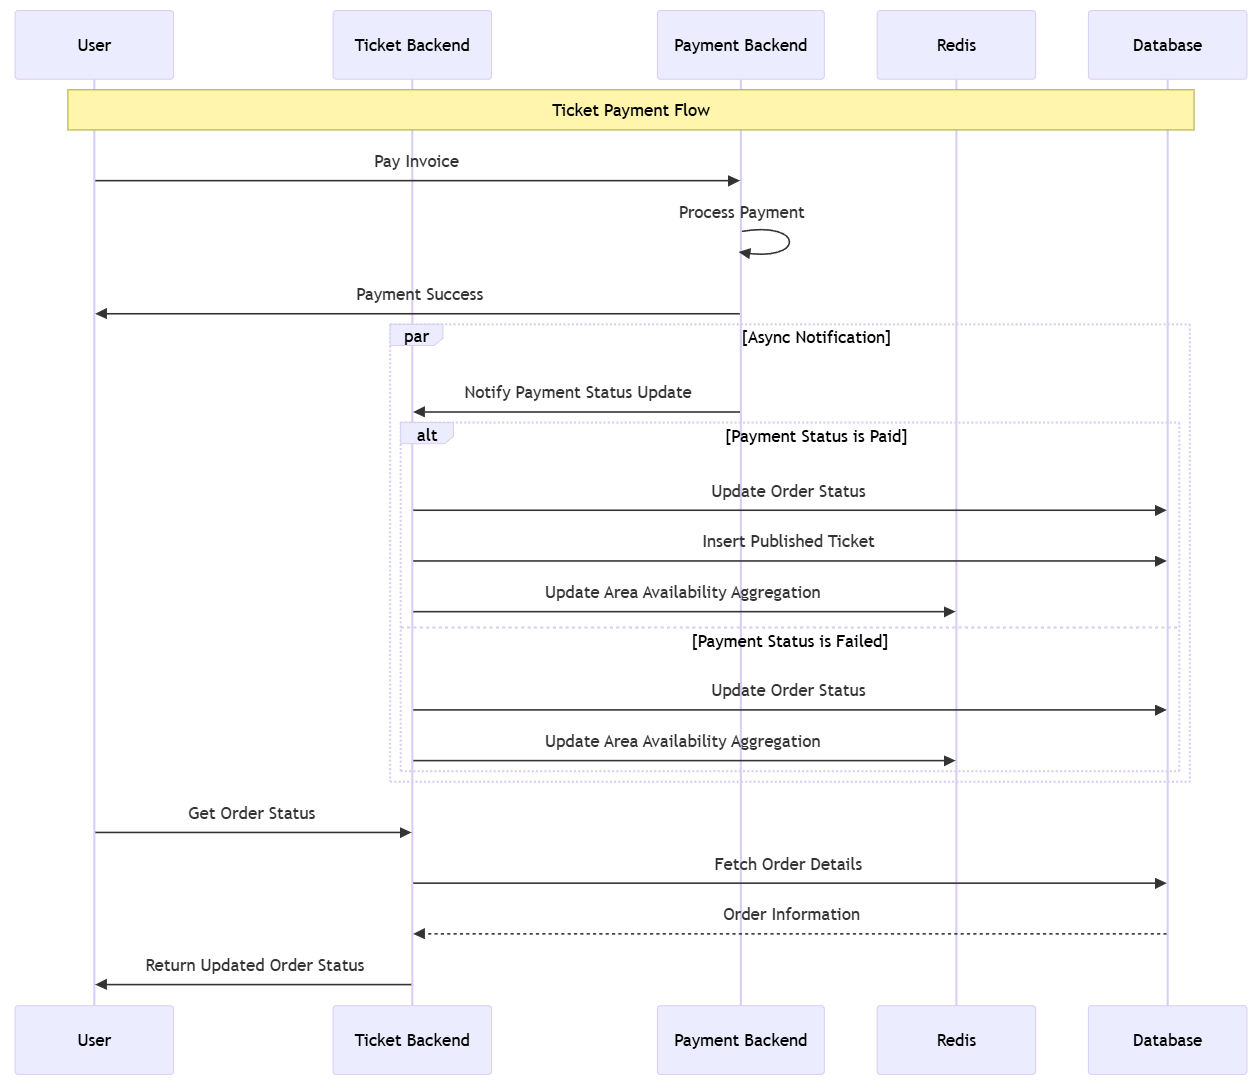
\includegraphics[width=1\textwidth]{resources/chapter-3/order-payment.png}
    \caption{Diagram Alur Fitur Pembayaran Tiket (tanpa \textit{flow control})}
    \label{fig:flow-order-payment-fc}
\end{figure}

\pagebreak

\subsubsection{Alur Fitur Pembacaan Pesanan}

Terdapat dua operasi tambahan yang berkaitan dengan pembacaan pesanan, yaitu membaca detail pesanan dan membaca tiket yang sudah diterbitkan.

\begin{figure}[h]
    \centering
    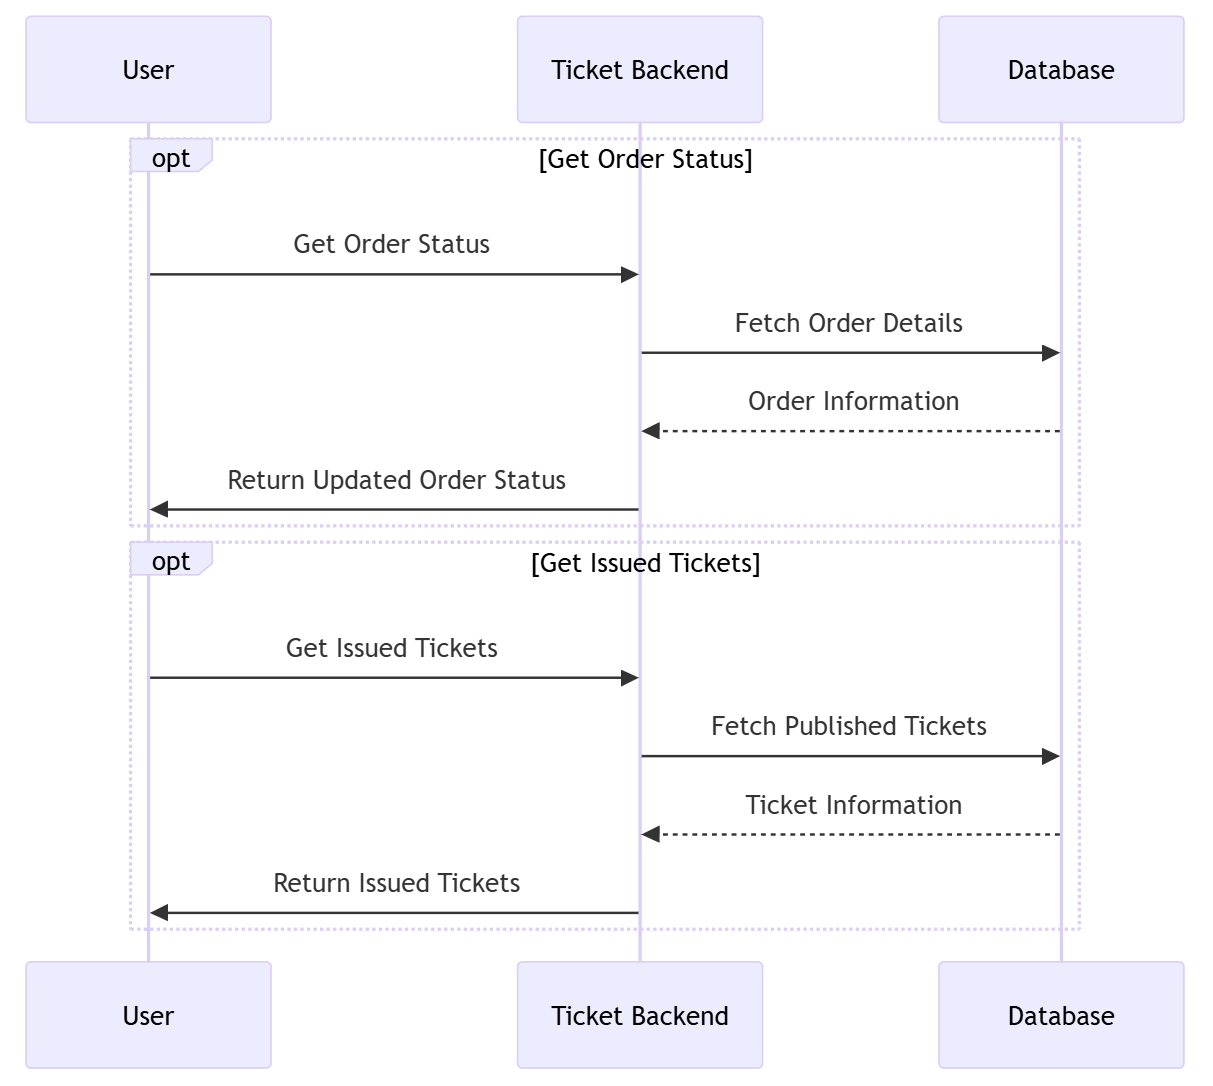
\includegraphics[width=1\textwidth]{resources/chapter-3/order-flow.png}
    \caption{Diagram Alur Fitur Pembacaan Pesanan}
    \label{fig:flow-order-flow}
\end{figure}